\section{{\tool}: Approach Overview}
\label{overview:sec}

%{\tool} has two main processes: training and predicting.


\subsection{Training Process}

Figure~\ref{overview-training} shows the overview of our training
process. If a method has multiple buggy statements, we treat one buggy
statement at a time and its enclosing method, together with its
respective fixed code as an input training instance.
%The input of~this process is the source code of a buggy method and one
%of its buggy statements, and the respective fixed source code.
The output includes the trained CCL model and the trained CTL model.
The training process has two main steps:

\begin{figure}[t]
	\centering
	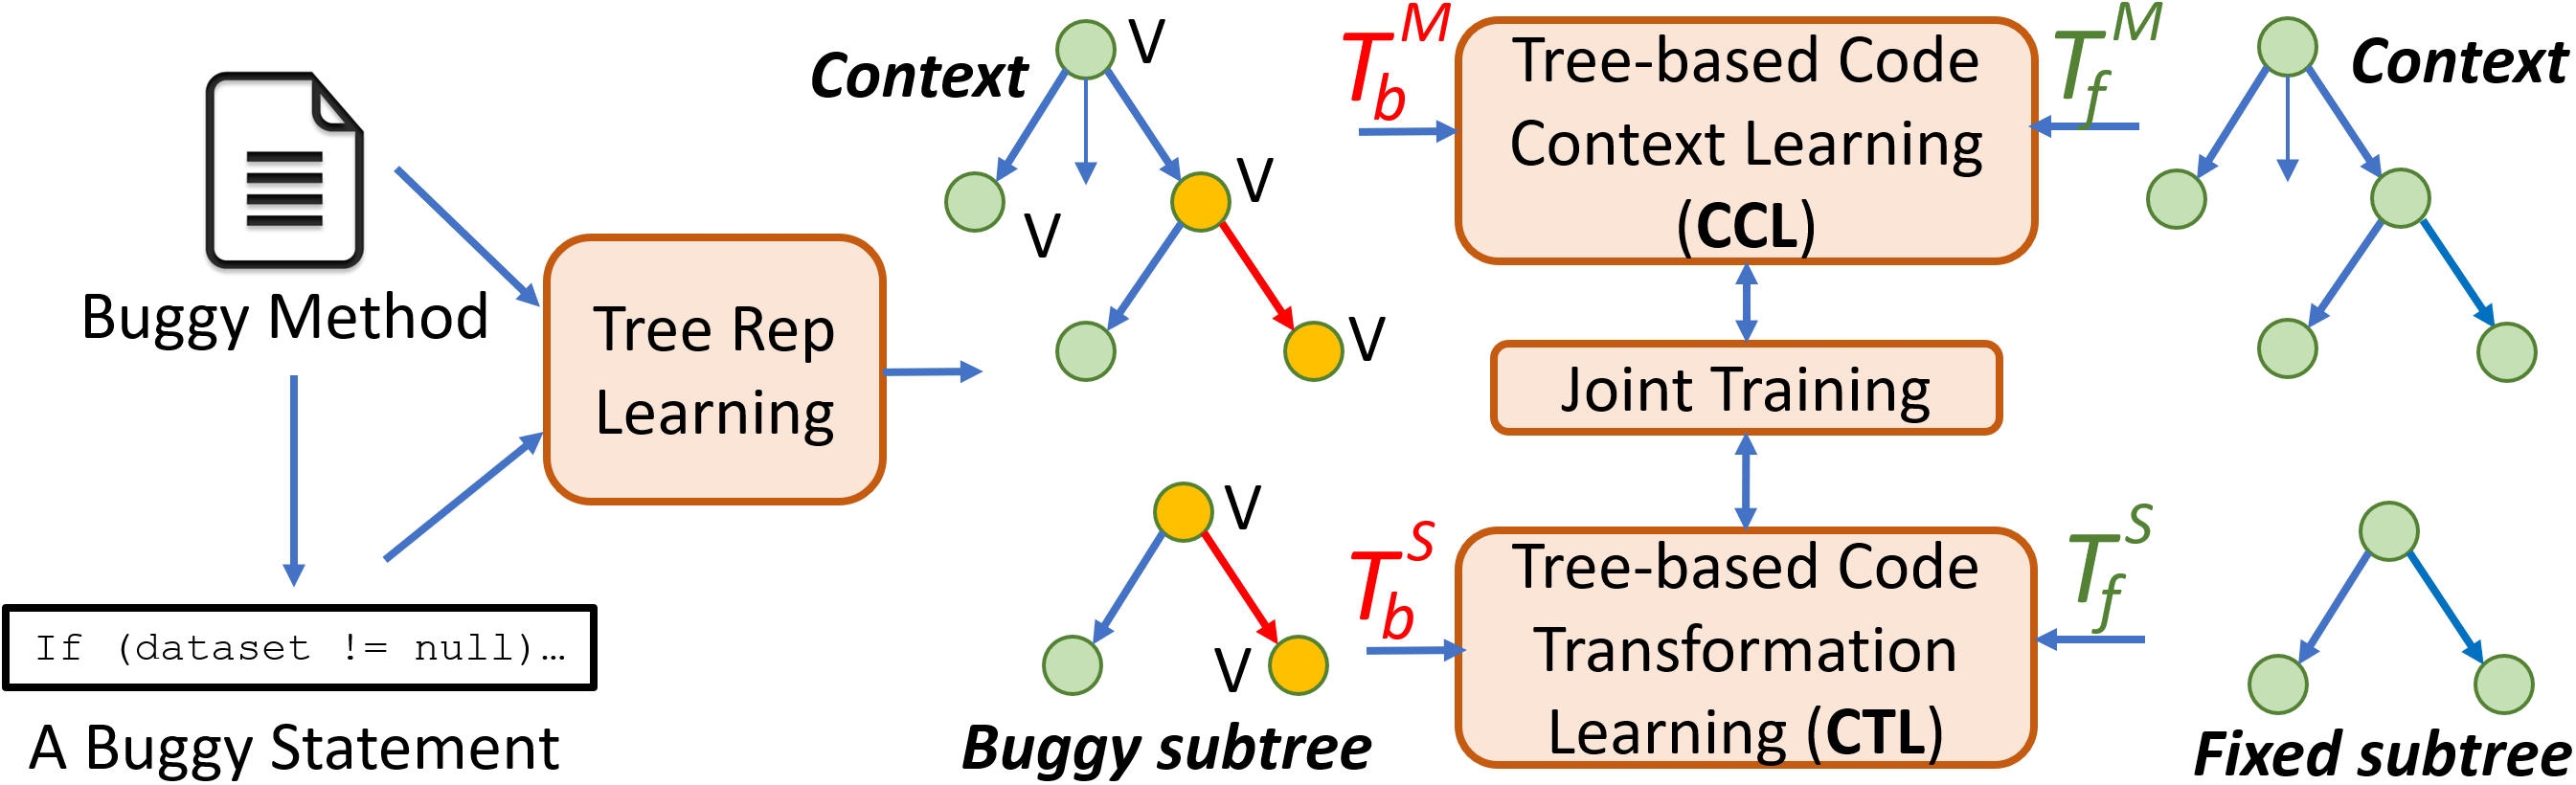
\includegraphics[width=3.4in]{graphs/new_overview-4.png}
%        \vspace{-9pt}
	\caption{{\tool}: Training Process}
	\label{overview-training}
%	\vspace{-10pt}
\end{figure}

%\vspace{2pt}
%\noindent {\bf Tree-based Representation Learning.}

\subsubsection{Tree-based Representation Learning}

{\tool} takes the source code and builds the vectors to be the inputs
of CCL and CTL. To achieve that, the given method is parsed to obtain
its AST and the subtree for the buggy statement.  Then, a word
embedding technique is used to produce the vector for each node in the
AST when we flatten the AST into a sequence. After this, we obtain the
AST for the method and the AST subtree for the buggy statement in
which {\em each node is replaced by its embedding vector}.

To build the context, we leverage the known buggy statement $s$ by
collecting the AST nodes that have {\em data and control dependencies
  with $s$}. We then take the subtree that covers all
those nodes and use it as the context
(Figure~\ref{overview-training}). This subtree $T_b^{M}$ is used as
the input for the Code Context Learning model (CCL) in the later step.

For code-transformation learning, we use the AST subtree $T_b^{S}$ for
the buggy statement with the embedding vectors as the input for the
Code Transformation Learning model (CTL) in the next step.

%\vspace{2pt}
%\noindent {\bf Context-aware, Dual-Task Learning Automated Program Repair.}

\subsubsection{Context-aware, Dual-Task Learning Automated Program
  Repair}

The goal of this step is to train both the tree-based CCL and the
tree-based CTL in a joint-training manner. For CCL, the context AST
(with the embeddings) before the fix is used in the input layer and
the corresponding context AST after the fix is used in the output
layer of the CCL model. For CTL, the buggy subtree with the embeddings
is used in the input layer and the corresponding fixed subtree is used
in the output layer of the CTL model.
%The entire AST $T^{M}_b$ of the buggy method after vectorization
%(i.e., each node is a vector) is used at the input layer of CCL for
%training. The AST of the corresponding fixed method $T^{M}_f$ after
%vectorization is used at the output layer of CCL. Similarly, the AST
%subtree $T^{S}_b$ of the buggy statement after vectorization is used
%at the input layer of CTL, and the subtree $T^{S}_f$ of the
%corresponding fixed statement after vectorization is used at the
%output layer of CTL.

The CCL and CTL models are realized via attention-based \code{seq2seq}
models. We use the {\em cross-stitch unit}~\cite{misra2016cross} to
train CCL and CTL simultaneously (Section~\ref{sec: dual-learning}).
%with soft-sharing the parameters to exploit this duality.
Joint training is aimed to learn the shared representations between
CCL amd CTL in terms of a linear combination of the input features in
both models.  The output includes the trained CCL and CTL models.

\subsection{Prediction Process}

\begin{figure}[t]
	\centering
	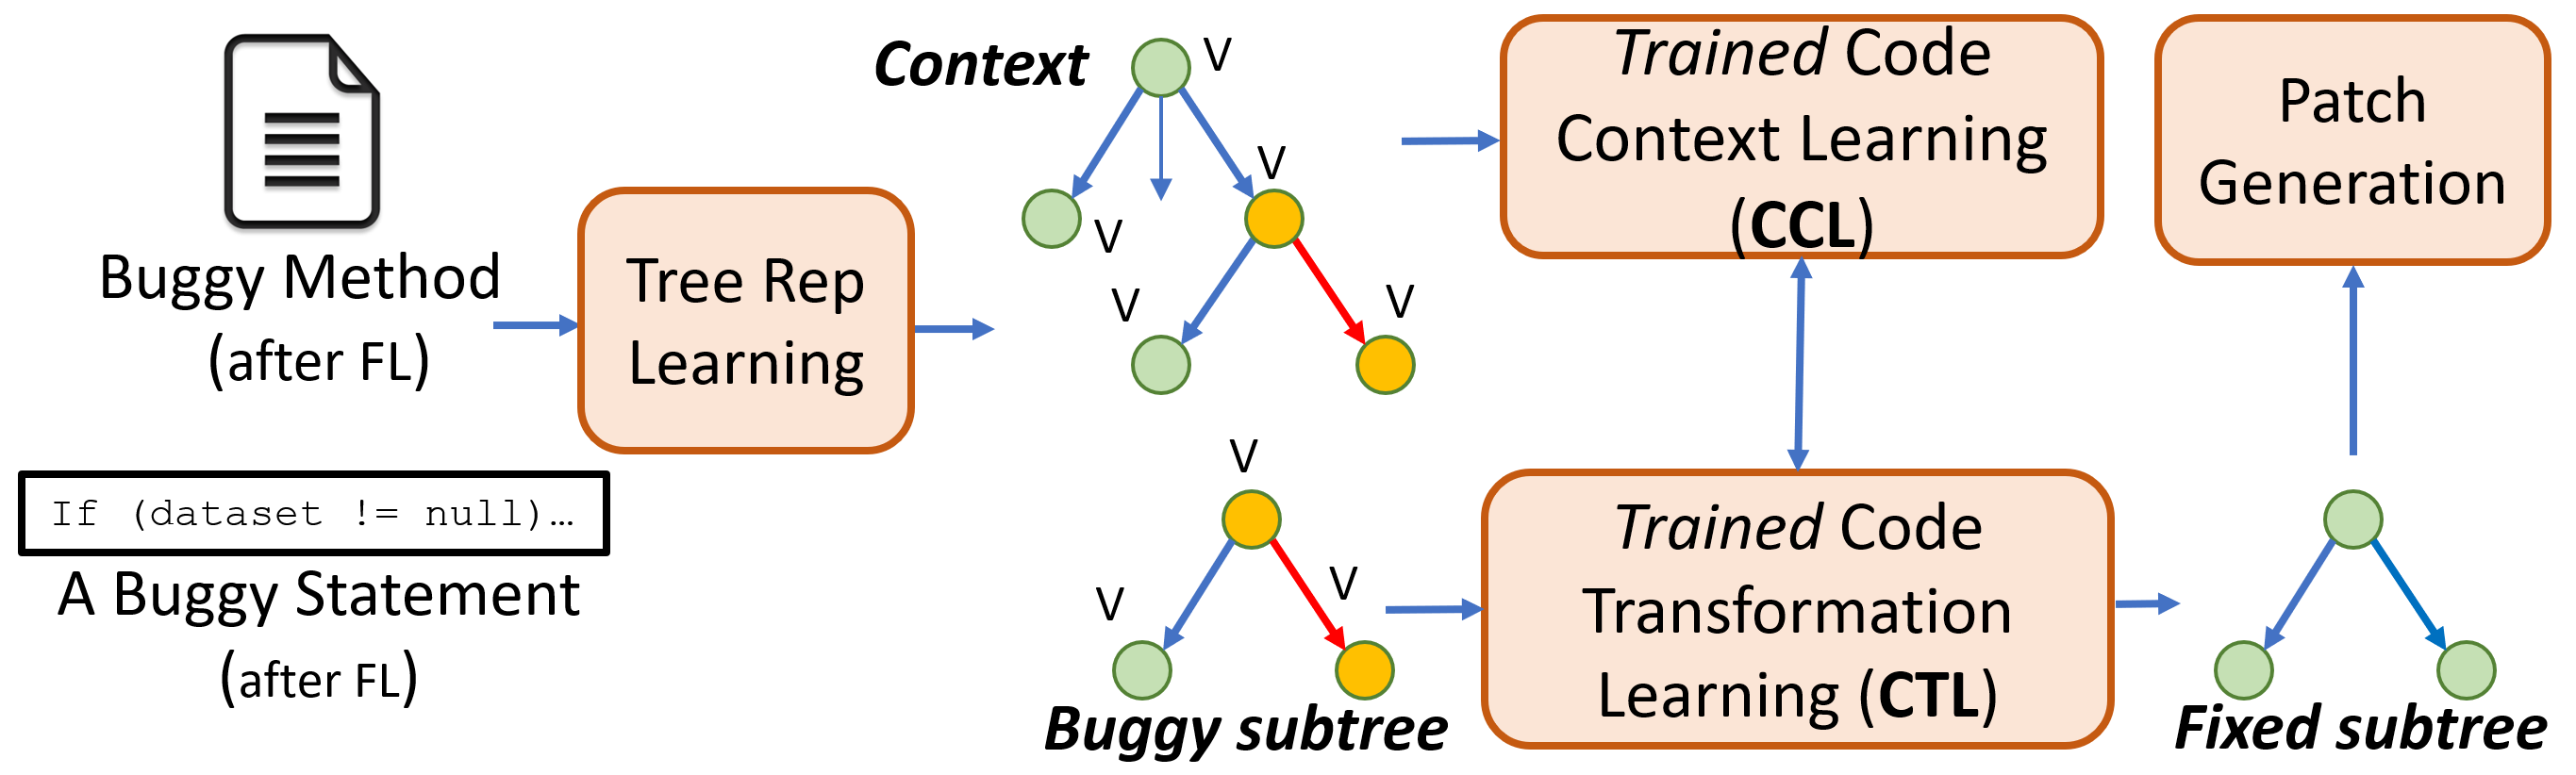
\includegraphics[width=3.4in]{graphs/overview-predict-4.png}
	\caption{{\tool}: Fixing Process}
        \vspace{-3pt}
	\label{overview-fixing}
\end{figure}

Figure~\ref{overview-fixing} illustrates the prediction process, i.e.,
the automated fixing process. A common usage of our tool is that
a developer could first use a fault localization tool
(FL) to detect the buggy statements that need to be fixed. Then, the
input for {\tool} is a buggy statement in the enclosing method.
%Another usage is that a developer can pinpoint the buggy statement and
%invoke {\tool} for an auto-fixing suggestion.
The fixing process shares the first step of Tree-based Representation
Learning with the training process.

After that step, the vectorized buggy AST subtree (a node is replaced
by a vector), is used as the input of the trained CTL model. The
output of the trained CTL model is the fixed AST subtree, which is
converted back into source code to form a candidate patch. We use a
patch generation that uses beam search over the AST structure and
works in accordance with the decoder as part of CTL to improve
efficiency (Section~\ref{sec:patch-gen}). Finally, we adopt the patch
validation process via test cases as in test-based APR~\cite{icse20}.

%the candidate patches are validated and output.

%We design a novel patch validation scheme that makes use of beam
%search for an efficient process. The final candidate patches are then
%produced.


